%!TEX root = main.tex
\newpage
\chapter{StackLetter -- personalizovaný informačný bulletin pre Stack Exchange}

\textit{StackLetter} je systém pre vytváranie a rozosielanie personalizovaných informačných bulletinov vrámci platformy
Stack Exchange. Tento systém vznikol sko súčasť spolupráce autora tejto práce a Bc. Matúša Saláta~\cite{Salat2018} vrámci
dvoch diplomových prác riešených v akademickom roku 2016/17 a 2017/18. Celý systém sa skladá
z viacerých spolupracujúcich modulov, ktoré však boli vyvíjané samostatne a sú od seba navzájom nezávislé. Rozdelenie
systému na nezávislé moduly umožňuje rýchlejší vývoj, ako aj možnosť jednoduchého rozširovania systému v budúcnosti.
Architektonický prehľad celého systému znázorňuje obrázok~\ref{fig:architecutre-overview}. Ďalej v tejto práci popisujem
len mnou navrhnuté moduly.

\begin{figure}[H]\begin{center}
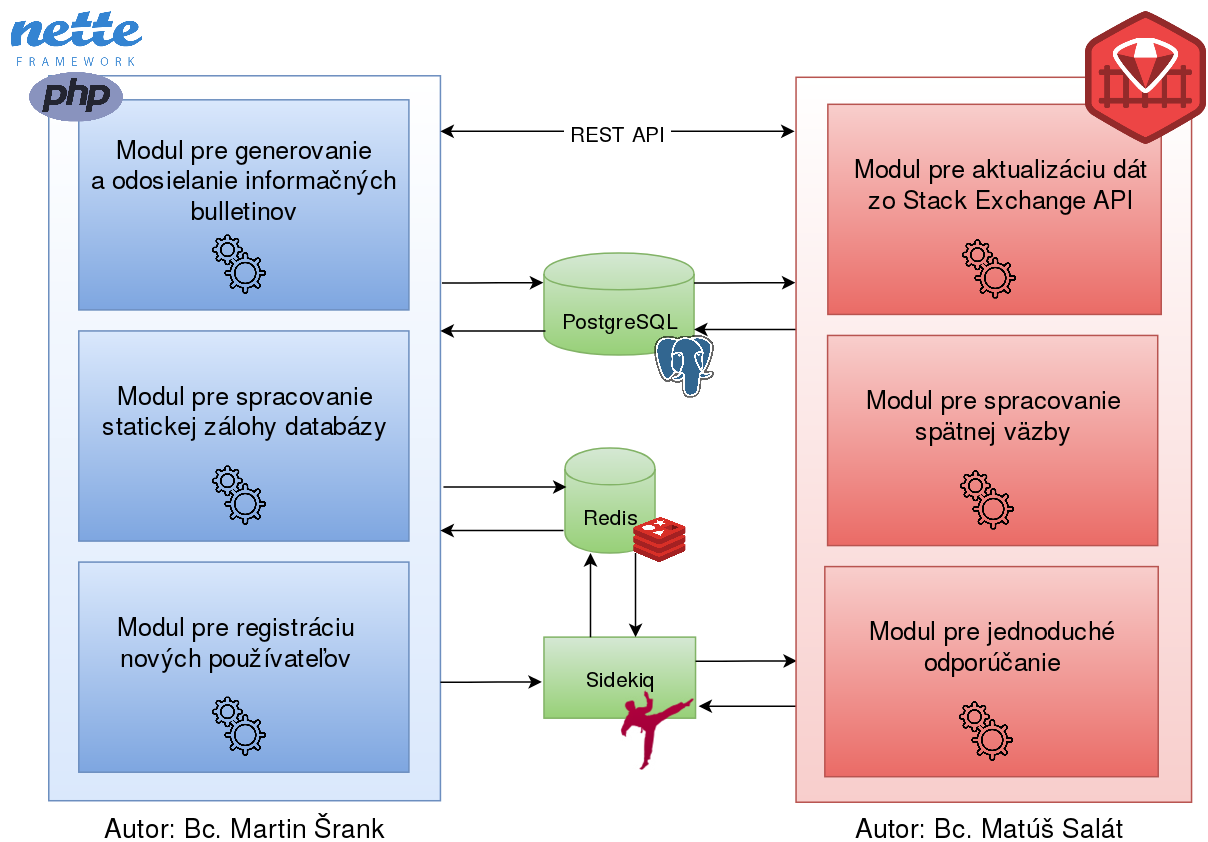
\includegraphics[scale=0.37]{architecture-overview}
\caption{Architektonický prehľad systému StackLetter. \label{fig:architecutre-overview}}\end{center}
\end{figure}

\section{Prehľad modulov}

\textbf{Modul pre registráciu nových používateľov}\\
Tento modul predstavuje používateľmi viditeľnú časť systému. Prostredníctvom webovej stránky systému
-- \url{www.stackletter.com} -- sa používatelia môžu prihlásiť k odoberaniu informačného bulletinu pre niektoré
z ponúkaných komunít platformy Stack Exchange, ako aj spravovať svoje nastavenia týkajúce sa odosielania informačných
bulletinov.\\
Používatelia sa prihlasujú prostredníctvom svojho Stack Exchange konta využitím protokolu OAuth.

\begin{figure}[H]\begin{center}
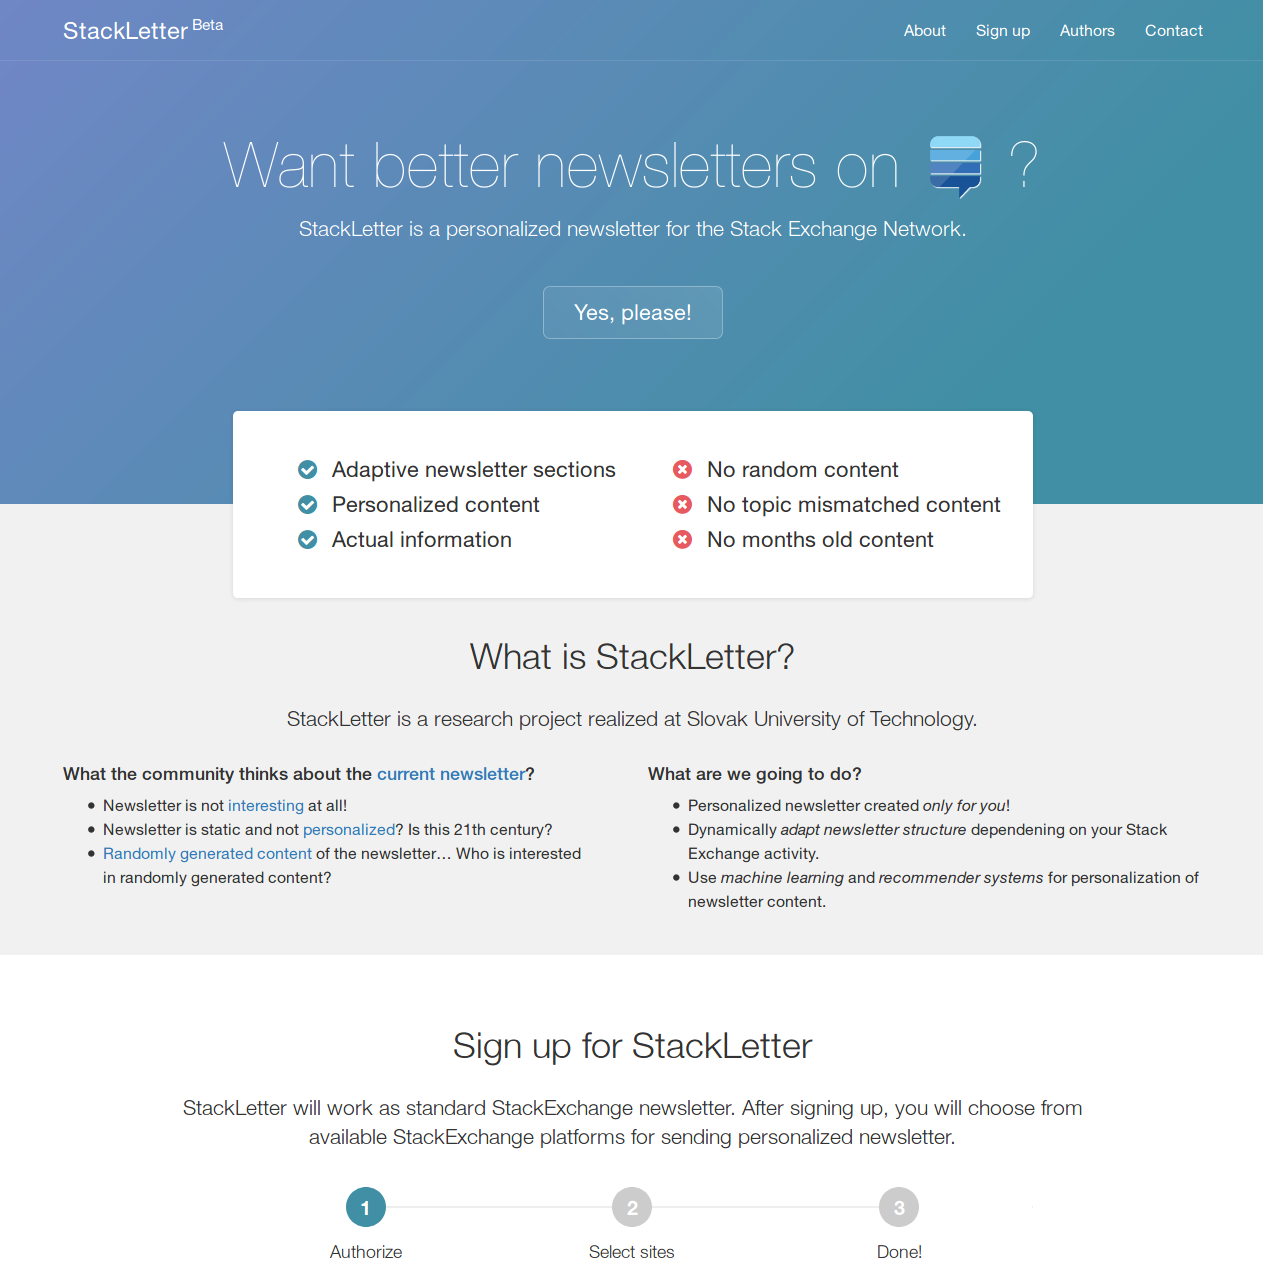
\includegraphics[scale=0.25]{stackletter-screenshot}
\caption{Snímka registračnej stránky StackLetter.com. \label{fig:stackletter.com}}\end{center}
\end{figure}

\textbf{Modul pre generovanie a odosielanie informačných bulletinov}\\
Tento modul je zodpovedný za samotné zostavovanie a odosielanie informačných bulletinov jednotlivým zaregistrovaným
používateľom. Prostredníctvom REST API komunikuje s modulmi pre zostavovanie odporúčaní a štruktúry informačných bulletinov
a na základe ich odpovedí vygeneruje naformátované informačné bulletiny, ktoré sú následne rozosielané prostredníctvom služby
SendGrid\footnote{\url{https://sendgrid.com}}.

\textbf{Modul pre spracovanie statickej zálohy databázy}\\
Modul bol navrhnutý a implementovaný za účelom rýchleho a efektívneho importovania počiatočných dát platformy Stack Exchange
dostupných vo forme XML exportu do našej internej reprezentácie v databáze PostgreSQL.

Podrobný technický a architektonický popis jednotlivých modulov sa nachádza
v prílohe~\ref{tech-doc} -- \textit{Technická dokumentácia systému StackLetter}.

\section{Použité technológie a služby}

\begin{my_itemize}
\item{Jednotlivé moduly zabezpečujúce infraštruktúru systému StackLetter sú implementované v~jazyku PHP\footnote{\url{https://php.net}}
verzie~7.1 s použitím MVC frameworku Nette~2.4\footnote{\url{https://nette.org}}.}
\item{Systém na ukladanie dát využíva relačný databázový systém PostgreSQL vo verzii 9.6 a vnútropamäťové dátové úložisko Redis
vo verzii 4.0.}
\item{Systém komunikuje s platformou Stack Exchange prostredníctvom Stack Exchange API v2.2 a~vykonáva autentifikáciu
používateľov prostredníctvom protokolu OAuth 2.0.}
\item{Na hromadné odosielanie informačných bulletinov používateľom prostredníctovm e-mailu je využitá služba SendGrid.}
\item{Modul implementujúci zostavovanie personalizovaných informačných bulletinov so zameraním na diverzitu bude implementovaný
v jazyku Python 3.6.}
\end{my_itemize}
